\documentclass{standalone}
\usepackage{tikz}

\begin{document}

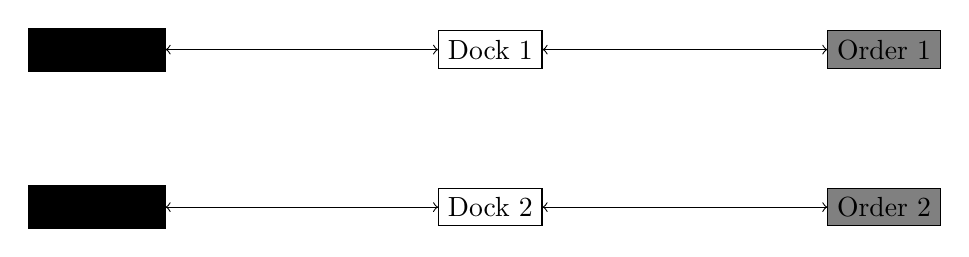
\begin{tikzpicture}[node distance=2cm]
    % Nodes representing dock approaches
    \node (dock1) [rectangle, draw, fill=white, text centered] {Dock 1};
    \node (dock2) [rectangle, draw, fill=white, text centered, below of=dock1] {Dock 2};

    % Nodes representing unloading and loading orders
    \node (order1) [rectangle, draw, fill=gray, text centered, right of=dock1, xshift=3cm] {Order 1};
    \node (order2) [rectangle, draw, fill=gray, text centered, right of=dock2, xshift=3cm] {Order 2};

    % Node representing waiting for ports to become free
    \node (waiting1) [rectangle, draw, fill=black, text centered, left of=dock1, xshift=-3cm] {Waiting 1};
    \node (waiting2) [rectangle, draw, fill=black, text centered, left of=dock2, xshift=-3cm] {Waiting 2};

    % Arrows connecting nodes
    \draw[->] (dock1) -- (order1);
    \draw[->] (dock2) -- (order2);
    \draw[->] (order1) -- (dock1);
    \draw[->] (order2) -- (dock2);
    \draw[->] (dock1) -- (waiting1);
    \draw[->] (dock2) -- (waiting2);
    \draw[->] (waiting1) -- (dock1);
    \draw[->] (waiting2) -- (dock2);
\end{tikzpicture}

\end{document}